\section{Attestation}
\begin{frame}
    \frametitle{Attestation}
    \begin{itemize}[<+->]
        \item Attestation is used to verify the integrity of an enclave:
        \begin{itemize}[<+->]
            \item Verifies that the code is trustable
            \item That the enclave code has not been tampered with
        \end{itemize}
        \item Enclaves can provide a report containing (excerpt):
        \begin{itemize}
            \item Enclave measurement (MRENCLAVE)
            \item Version numbers / IDs
            \item Authors identity
        \end{itemize}
        \item Report can be requested:
        \begin{itemize}
            \item By another enclave (local attestation)
            \item From another system (remote attestation)
        \end{itemize}
    \end{itemize}
\end{frame}

\begin{frame}
    \frametitle{Local Attestation}
    \begin{enumerate}[<+->]
        \item Enclave B request report from enclave A
        \item Enclave A creates report structure from using EREPORT instruction
        \item Report is generated by SGX using:
        \begin{itemize}
            \item Data from A's SECS-structure
            \item Message Authentication Code (MAC) over all report fields
        \end{itemize}
        \item Report is sent to enclave B
        \item B verifies Report using EGETKEY instruction
    \end{enumerate}
\end{frame}

\incfuck[\textwidth]{LocalAttestation}{1}{}{Local Attestation}
\incfuck[\textwidth]{LocalAttestation}{2}{}{Local Attestation}
\incfuck[\textwidth]{LocalAttestation}{3}{}{Local Attestation}
\incfuck[\textwidth]{LocalAttestation}{4}{}{Local Attestation}
\incfuck[\textwidth]{LocalAttestation}{5}{}{Local Attestation}
\incfuck[\textwidth]{LocalAttestation}{6}{}{Local Attestation}

\begin{frame}
    \frametitle{Remote Attestation}
    \begin{columns}
        \begin{column}{0.4\textwidth}
            \begin{enumerate}[<+->]
                \item Application receives an attestation request from challenger
                \item Application requests report
                \item Application receives report
                \item Report is send to quoting enclave (QE)
                \item QE converts local report to remote report (Quote) and sends back
                \item Challenger receives quote
                \item Attestation verification service verifies quote
            \end{enumerate}
        \end{column}
        \begin{column}{0.6\textwidth}
            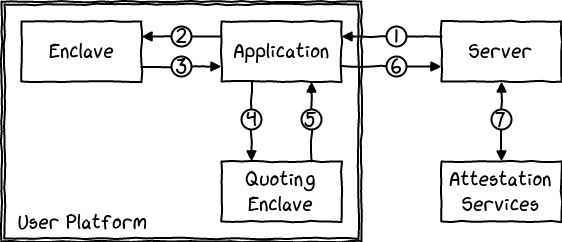
\includegraphics[scale=0.4]{Images/remote_attestation.png}
        \end{column}
    \end{columns}
\end{frame}

\section{Sealing}

\begin{frame}
    \frametitle{Sealing}
    \begin{itemize}[<+->]
        \item Secrets of an enclave gets lost when enclave is closed
        \item Process of encrypting enclave secrets for persistent storage is called sealing
        \item The data can be signed with different keys
        \item Enclave retrieves the sealing key using the EGETKEY instruction, which returns a cryptographic key
        \item Enclaves can seal data with MRENCLAVE as key, so no other enclave is able to read data
        \item Other key is MRSIGNER, so every enclave with same author can read each others data
    \end{itemize}
\end{frame}